\documentclass{beamer}
\usetheme{default}
\setbeamertemplate{navigation symbols}{}

\title{Ronald: A Multithreaded Path Tracing Renderer}
\subtitle{SENG 475 Final Project}
\author{Jayden Chan}
\institute{\href{https://github.com/jayden-chan/ronald}{https://github.com/jayden-chan/ronald}}
\date{August 15 2022}

\begin{document}

\begin{frame}
\titlepage
\end{frame}

\begin{frame}{What is Path Tracing?}
    \begin{itemize}[<+->]
        \item Computer graphics technique for creating photo realistic renderings
        \item Monte Carlo integration
        \item Based on the physical characteristics of light and the world (PBR)
        \item Very slow
    \end{itemize}
\end{frame}

\begin{frame}{What is Path Tracing?}
    \begin{center}
        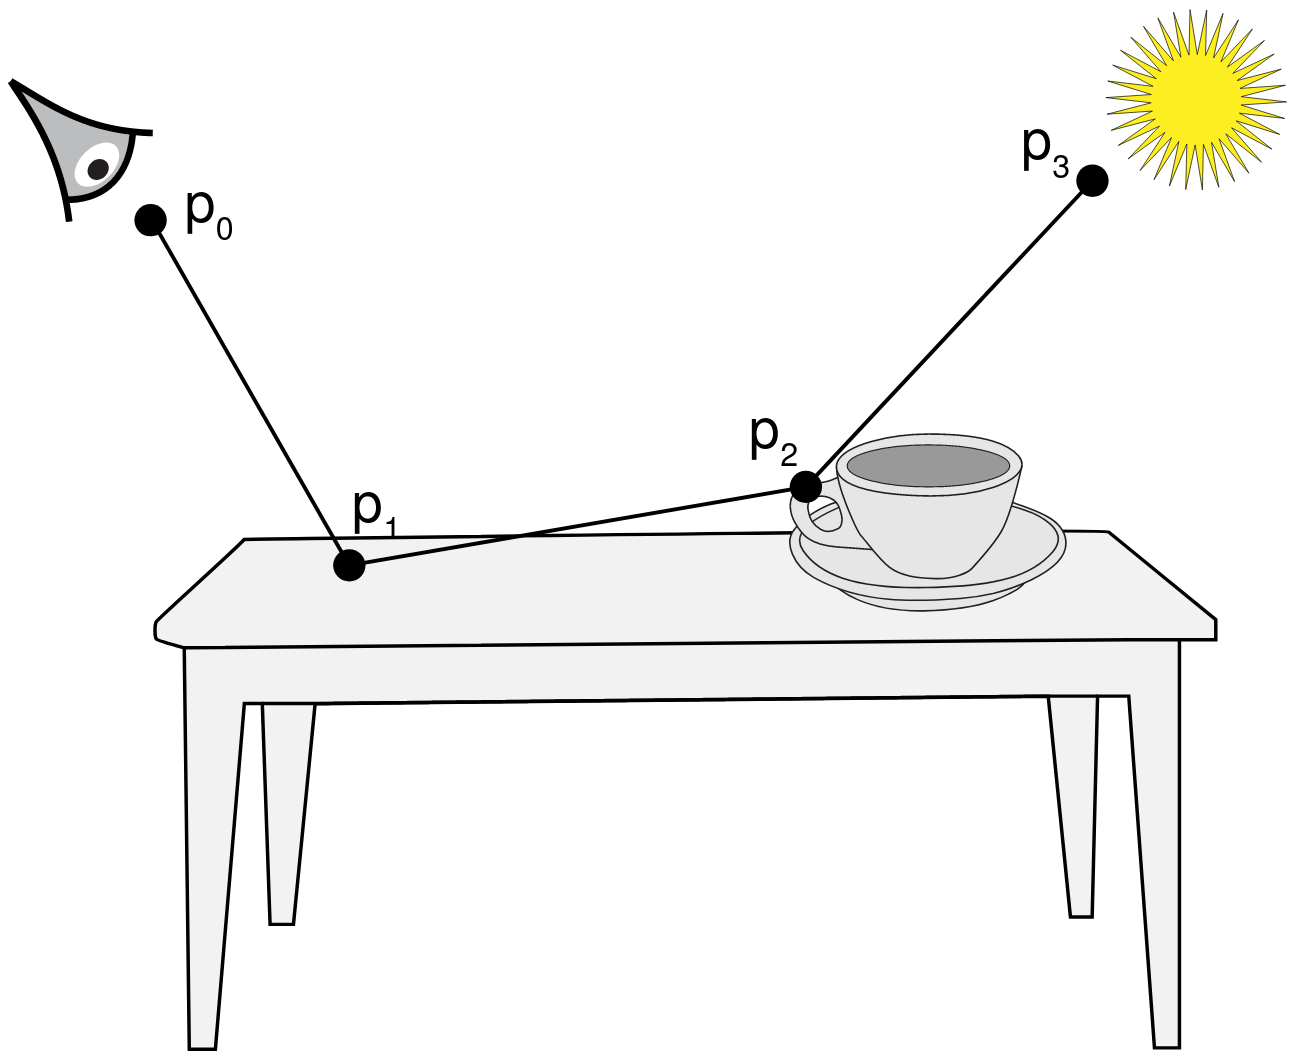
\includegraphics[width=0.9\textwidth]{./path_tracing.png}
    \end{center}
\end{frame}

\begin{frame}{Example: Monte Carlo Integration Convergence}
    Samples: 10
    \begin{center}
        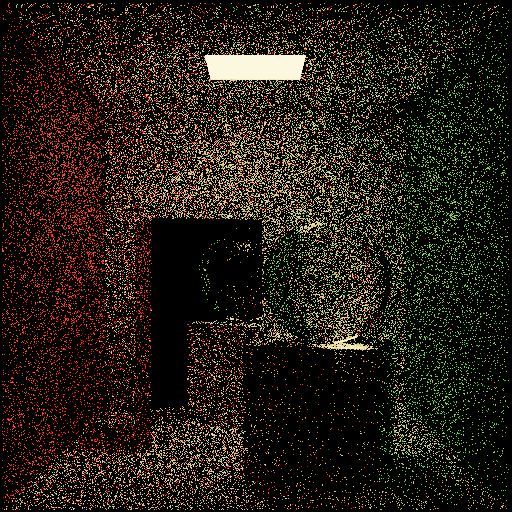
\includegraphics[width=0.65\textwidth]{../img/convergence/cornell-00010.png}
    \end{center}
\end{frame}

\begin{frame}{Example: Monte Carlo Integration Convergence}
    Samples: 25
    \begin{center}
        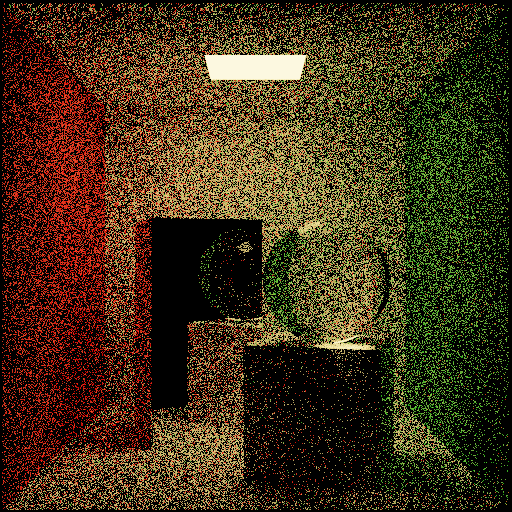
\includegraphics[width=0.65\textwidth]{../img/convergence/cornell-00025.png}
    \end{center}
\end{frame}

\begin{frame}{Example: Monte Carlo Integration Convergence}
    Samples: 50
    \begin{center}
        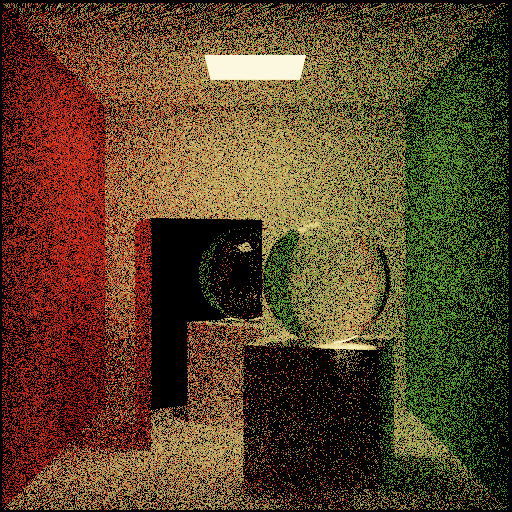
\includegraphics[width=0.65\textwidth]{../img/convergence/cornell-00050.png}
    \end{center}
\end{frame}

\begin{frame}{Example: Monte Carlo Integration Convergence}
    Samples: 100
    \begin{center}
        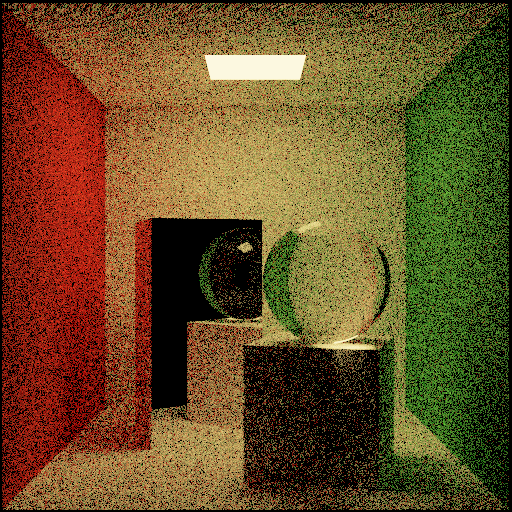
\includegraphics[width=0.65\textwidth]{../img/convergence/cornell-00100.png}
    \end{center}
\end{frame}

\begin{frame}{Example: Monte Carlo Integration Convergence}
    Samples: 200
    \begin{center}
        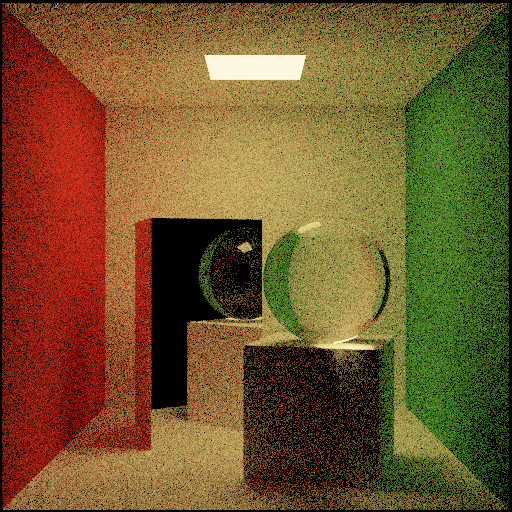
\includegraphics[width=0.65\textwidth]{../img/convergence/cornell-00200.png}
    \end{center}
\end{frame}

\begin{frame}{Example: Monte Carlo Integration Convergence}
    Samples: 500
    \begin{center}
        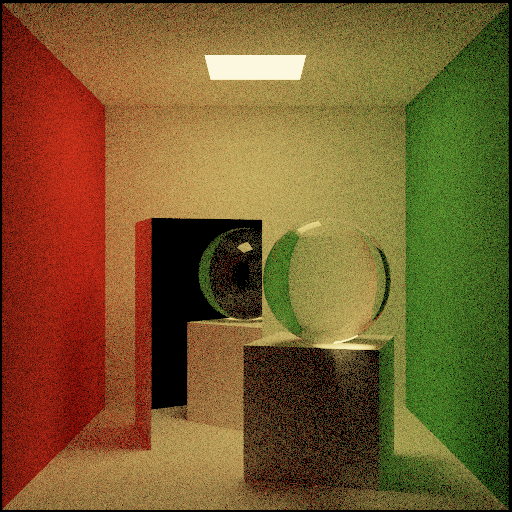
\includegraphics[width=0.65\textwidth]{../img/convergence/cornell-00500.png}
    \end{center}
\end{frame}

\begin{frame}{Example: Monte Carlo Integration Convergence}
    Samples: 1300
    \begin{center}
        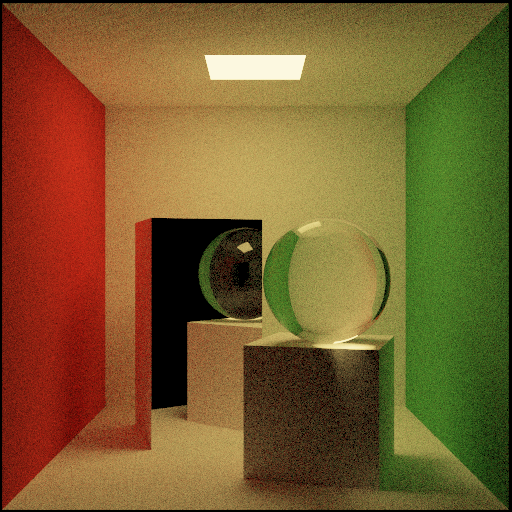
\includegraphics[width=0.65\textwidth]{../img/convergence/cornell-01300.png}
    \end{center}
\end{frame}

\begin{frame}{Example: Monte Carlo Integration Convergence}
    Samples: 3000
    \begin{center}
        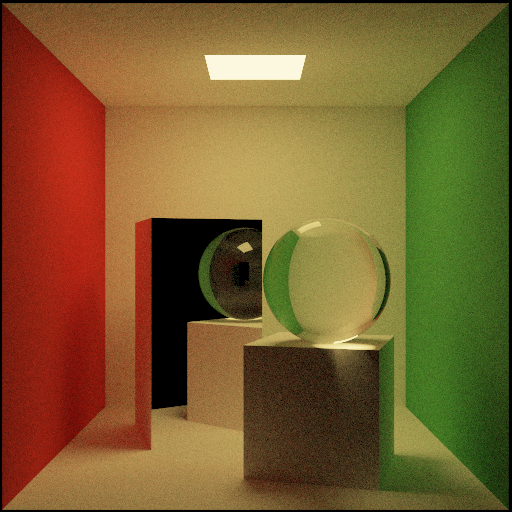
\includegraphics[width=0.65\textwidth]{../img/convergence/cornell-03000.png}
    \end{center}
\end{frame}

\begin{frame}{Example: Monte Carlo Integration Convergence}
    Samples: 15000
    \begin{center}
        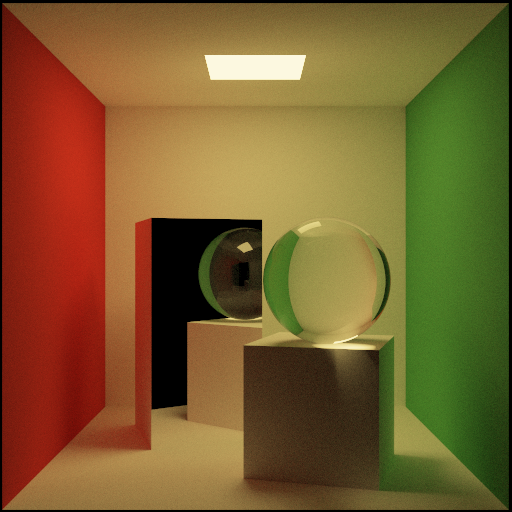
\includegraphics[width=0.65\textwidth]{../img/convergence/cornell-15000.png}
    \end{center}
\end{frame}

\end{document}
